% ============================================================
% 实验报告 —— 系统开发工具基础 · Week 1
% 包含四道题目：文件操作、日志分析、Git 分支合并、LaTeX 编译
% 编译方式: xelatex lab_report.tex （编译两次）
% ============================================================

\documentclass[12pt, a4paper]{article}

% ==================== 中文与字体 ====================
\usepackage{fontspec}
\usepackage{xeCJK}
\setCJKmainfont{仿宋}[AutoFakeBold=true, AutoFakeSlant=true]
\setmainfont{Cambria}

% ==================== 页面布局 ====================
\usepackage{geometry}
\geometry{
    a4paper,
    left=2.8cm,
    right=2.8cm,
    top=2.8cm,
    bottom=2.8cm,
    headheight=15pt
}

% ==================== 颜色系统 ====================
\usepackage{xcolor}
\definecolor{mainblue}{RGB}{0, 182, 255}
\definecolor{lightblue}{RGB}{200, 220, 240}
\definecolor{codegray}{RGB}{245, 245, 245}
\definecolor{keywordcolor}{RGB}{0, 0, 255}
\definecolor{stringcolor}{RGB}{163, 21, 21}
\definecolor{commentcolor}{RGB}{0, 128, 0}

% ==================== 页眉页脚 ====================
\usepackage{fancyhdr}
\pagestyle{fancy}
\fancyhf{}
\renewcommand{\headrulewidth}{0.8pt}
\renewcommand{\headrule}{\color{mainblue}\hrule width\textwidth height 0.8pt}
\fancyhead[L]{\textcolor{mainblue}{\textbf{系统开发工具基础 · Week 1}}}
\fancyhead[R]{\textcolor{mainblue}{\thepage}}
\fancyfoot[C]{\textcolor{gray}{\small 25020007096 · Xingrui Pan}}

% ==================== 章节标题样式 ====================
\usepackage{titlesec, titletoc}
\titleformat{\section}
    {\Large\bfseries\color{mainblue}}
    {\thesection}{1em}{}
    [{\titlerule[0.5pt]}]

\titleformat{\subsection}
    {\large\bfseries\color{mainblue!80!black}}
    {\thesubsection}{1em}{}

% ==================== 目录样式 ====================
\usepackage{tocloft}
\renewcommand{\cftsecfont}{\color{mainblue}\bfseries}
\renewcommand{\cftsubsecfont}{\color{mainblue!80!black}}
\renewcommand{\cftsecpagefont}{\color{mainblue}}

% ==================== 列表样式 ====================
\usepackage{enumitem}
\setlist[enumerate]{
    label=\color{mainblue}\arabic*.,
    ref=\arabic*,
    leftmargin=1.2cm,
    itemsep=2pt
}
\setlist[itemize]{
    label=\textcolor{mainblue}{\textbullet},
    leftmargin=1.2cm,
    itemsep=2pt
}

% ==================== 图表与浮动体 ====================
\usepackage{graphicx}
\usepackage{caption}
\usepackage{subcaption}
\usepackage{float}
\captionsetup{
    font=small,
    labelfont={bf,color=mainblue},
    labelsep=period
}

% ==================== 表格增强 ====================
\usepackage{array, booktabs, colortbl}
\newcolumntype{C}{>{\centering\arraybackslash}X}

% ==================== 代码高亮 ====================
\usepackage{listings}
\lstset{
    basicstyle=\ttfamily\small,
    keywordstyle=\color{keywordcolor}\bfseries,
    stringstyle=\color{stringcolor},
    commentstyle=\color{commentcolor}\itshape,
    backgroundcolor=\color{codegray},
    frame=single,
    frameround=tttt,
    framesep=5pt,
    breaklines=true,
    showspaces=false,
    showstringspaces=false,
    tabsize=4,
    numbers=left,
    numberstyle=\tiny\color{gray},
    captionpos=b,
    xleftmargin=2pt,
    xrightmargin=2pt
}

% ==================== 数学公式 ====================
\usepackage{amsmath, amssymb, bm}
\usepackage{mathtools}
\numberwithin{equation}{section}

% ==================== 超链接 ====================
\usepackage{hyperref}
\hypersetup{
    colorlinks=true,
    linkcolor=mainblue,
    citecolor=mainblue,
    urlcolor=mainblue
}

% ==================== 自定义盒子 ====================
\usepackage{tcolorbox}
\tcbuselibrary{skins,breakable}
\newtcolorbox{conclusionbox}{
    colback=mainblue!5,
    colframe=mainblue,
    arc=4pt,
    boxrule=1pt,
    title={\textcolor{mainblue}{\textbf{结论}}},
    fonttitle=\bfseries,
    drop fuzzy shadow=mainblue!50
}

% ==================== 自定义命令（请修改个人信息） ====================
\newcommand{\course}{系统开发工具基础 · Week 1}
\newcommand{\experiment}{实验报告}
\newcommand{\student}{潘星睿}           
\newcommand{\studentid}{25020007096}    
\newcommand{\instructor}{周小伟}   
\newcommand{\department}{计算机科学与技术学院}
\newcommand{\university}{中国海洋大学}
\newcommand{\reportdate}{\today}
\newcommand{\github}{https://github.com/HiyamaHina/-}
% ==================== 正文开始 ====================
\begin{document}

% ============================================================
% 封面
% ============================================================
\begin{titlepage}
\centering
\includegraphics[width=5cm]{OUC.png}\\[0.3cm]
{\LARGE \textbf{\university}}\\[0.2cm]
{\large \department}\\[0.5cm]
\textcolor{mainblue}{\rule{0.45\textwidth}{1.2pt}}\\[0.8cm]
{\Huge \textbf{《\course》}}\\[0.3cm]
{\large \experiment}\\[1.2cm]

\begin{minipage}{0.6\textwidth}
\centering
\setlength{\extrarowheight}{4pt}
\begin{tabular}{r l}
    \textcolor{mainblue}{\textbf{姓　　名}} & \student \\
    \textcolor{mainblue}{\textbf{学　　号}} & \studentid \\
    \textcolor{mainblue}{\textbf{指导教师}} & \instructor \\
    \textcolor{mainblue}{\textbf{日　　期}} & \reportdate \\
    \textcolor{mainblue}{\textbf{GitHub仓库}} & \github
\end{tabular}
\includegraphics[width=10cm]{AGLY.png}\\[0.3cm]
\end{minipage}

\vfill
\end{titlepage}

% ============================================================
% 摘要
% ============================================================
\newpage
\section*{摘要}
\addcontentsline{toc}{section}{摘要}
本次实验涵盖四个独立任务：Shell 文件操作、日志统计分析、Git 版本控制与分支合并、以及 LaTeX 文档编译。通过这些任务，巩固了 Linux 命令行、正则表达式、版本管理以及科技排版的基本技能。

\vspace{0.5cm}
\textbf{关键词：} Shell入门；VersionControl and Git；LaTeX 文档编辑\\
本次试验github的commit记录如下：\\
\includegraphics[width=15cm]{Git.png}\\[0.3cm]

% ============================================================
% 目录
% ============================================================
\newpage
\tableofcontents
\newpage

% ============================================================
% 第1题
% ============================================================
\section{第1题：文件与目录操作}
\label{sec:q1}

\subsection{题目要求}
在 \texttt{q01} 目录下完成以下操作：
\begin{enumerate}
    \item 创建目录结构 \texttt{input/docs} 和 \texttt{input/tmp}。
    \item 创建文件：\texttt{input/docs/notes one.txt}（内容为 alpha 和 beta），\texttt{input/docs/.secret.txt}（内容为 hidden），\texttt{input/tmp/empty.txt}（空文件），\texttt{input/run.log}（任意两行日志）。
    \item 显示 \texttt{q01} 的绝对路径，并以长格式列出 \texttt{input} 下全部项目（含隐藏文件）。
    \item 将所有 \texttt{.txt} 文件复制到 \texttt{work/<学号>/}，保留相对目录结构并正确处理空格。
    \item 设置目录权限为 750，普通文件权限为 640，生成 \texttt{inventory.txt} 列出相对路径和字节数。
\end{enumerate}

\subsection{实现过程}
使用 Shell 命令完成上述任务。关键命令如下：
\begin{lstlisting}[language=bash, caption=目录创建与文件生成]
mkdir -p input/docs input/tmp
echo -e "alpha\nbeta" > "input/docs/notes one.txt"
echo "hidden" > "input/docs/.secret.txt"
touch input/tmp/empty.txt
echo -e "2026-08-24 10:00:01 Start\n2026-08-24 10:00:02 End" > input/run.log
\end{lstlisting}

文件复制时使用 \texttt{find} 配合 \texttt{while read} 处理文件名中的空格：
\begin{lstlisting}[language=bash, caption=保留目录结构的复制]
find input -name "*.txt" -type f | while IFS= read -r file; do
    rel="${file#input/}"
    dest="work/$STUDENT_ID/$rel"
    mkdir -p "$(dirname "$dest")"
    cp "$file" "$dest"
done
\end{lstlisting}

\subsection{踩坑记录}
\begin{enumerate}
    \item \textbf{文件名空格处理：} 最初直接使用 \texttt{cp input/docs/notes one.txt dest/}，没有加引号，Shell 将 \texttt{notes} 和 \texttt{one.txt} 识别为两个独立的参数，导致命令失败。解决方法：将文件名用双引号括起来，如 \texttt{"notes one.txt"}。
    \item \textbf{\texttt{find} 与 \texttt{while read} 的配合：} 一开始尝试用 \texttt{for file in \$(find input -name "*.txt")}，当文件名包含空格时会被拆分成多个单词。改用 \texttt{find ... -print0 | while IFS= read -r -d '' file} 后问题解决。
    \item \texttt{filelist.txt} 缺失 \texttt{notes one.txt}：先执行 \texttt{find} 生成文件列表，再创建 \texttt{notes one.txt}，导致列表中没有该文件。解决方法：先创建所有文件，再执行 \texttt{find}。
    \item \texttt{IFS} 拼写错误：将 \texttt{IFS} 误写为 \texttt{IFE}，导致 \texttt{-r: command not found} 错误。修正后正常执行。
\end{enumerate}

\subsection{验证结果}
执行后，\texttt{work/学号/} 下应包含三个文件，权限设置正确，\texttt{inventory.txt} 列出所有文件及其大小。截图如下\\
\includegraphics[width=15cm]{q01.png}\\[0.3cm]\\

% ============================================================
% 第2题
% ============================================================
\section{第2题：日志统计分析}
\label{sec:q2}

\subsection{题目要求}
在 \texttt{q02} 中创建 \texttt{access.csv}，编写 \texttt{analyze.sh} 脚本：
\begin{enumerate}
    \item 接收一个 CSV 文件路径，文件不存在时输出错误到 stderr 并返回非零退出码。
    \item 输出 HTTP 5xx 数量最多的前 2 个 path，按次数降序，次数相同按 path 字典序。
    \item 输出全部数据行的平均 \texttt{latency\_ms}，保留两位小数，表头不计入。
    \item 分别对 \texttt{access.csv} 和不存在的文件运行脚本。
\end{enumerate}

\subsection{数据内容}
\begin{table}[H]
\centering
\caption{\texttt{access.csv} 数据样例}\label{tab:q2data}
\begin{tabular}{|c|c|c|c|c|}
\hline
\textbf{timestamp} & \textbf{user} & \textbf{path} & \textbf{status} & \textbf{latency\_ms} \\
\hline
09:00:01 & alice & /api/users & 200 & 120 \\
09:00:02 & bob & /api/orders & 500 & 310 \\
09:00:03 & alice & /api/users & 503 & 180 \\
09:00:04 & carol & /login & 500 & 90 \\
09:00:05 & bob & /api/orders & 502 & 260 \\
09:00:06 & dave & /health & 200 & 20 \\
09:00:07 & alice & /api/orders & 500 & 420 \\
09:00:08 & carol & /api/users & 500 & 150 \\
\hline
\end{tabular}
\end{table}

\subsection{实现过程}
核心管道命令如下：
\begin{lstlisting}[language=bash, caption=5xx 统计与平均延迟计算]
# 统计 5xx 最多的前 2 个 path
tail -n +2 access.csv | awk -F',' '$4 >= 500 && $4 < 600 {print $3}' | sort | uniq -c | sort -rn | head -2

# 计算平均延迟
tail -n +2 access.csv | cut -d',' -f5 | awk '{sum+=$1; count++} END {printf "%.2f", sum/count}'
\end{lstlisting}

\subsection{踩坑记录}
\begin{enumerate}
    \item \texttt{awk} 字段分隔符：CSV 文件使用逗号分隔，必须指定 \texttt{-F','}，否则 \texttt{awk} 默认以空格分隔，无法正确解析。    
\end{enumerate}

\subsection{运行结果}
对 \texttt{access.csv} 运行脚本后，输出如下：
\begin{verbatim}
=== Top 2 paths with most 5xx errors ===
/api/users 3
/api/orders 2
=== Average latency ===
193.75
\end{verbatim}

对不存在的文件运行，脚本输出错误信息并返回非零退出码。截图如下\\
\includegraphics[width=15cm]{q0201.png}\\[0.3cm]\\
\includegraphics[width=10cm]{q0202.png}\\[0.3cm]\\


% ============================================================
% 第3题
% ============================================================
\section{第3题：Git 分支与合并冲突}
\label{sec:q3}

\subsection{题目要求}
在 \texttt{q03} 中从零创建 Git 仓库，主动制造并解决一次合并冲突：
\begin{enumerate}
    \item 初始化仓库，在 \texttt{main} 创建 \texttt{config.txt}，内容为 \texttt{mode=normal}，完成初始提交。
    \item 创建 \texttt{feature-a}，改为 \texttt{mode=safe} 并提交；从初始 \texttt{main} 创建 \texttt{feature-b}，改为 \texttt{mode=fast} 并提交。
    \item 回到 \texttt{main}，先合并 \texttt{feature-a}，再合并 \texttt{feature-b}。
    \item 解决冲突时保留 \texttt{mode=safe}，并另加一行 \texttt{note=reviewed}。
    \item 确认工作区干净，运行 \texttt{git log --all --graph --decorate --oneline} 查看历史。
\end{enumerate}

\subsection{实现过程}
关键 Git 命令如下：
\begin{lstlisting}[language=bash, caption=Git 分支与合并]
git init
echo "mode=normal" > config.txt && git add . && git commit -m "Initial commit"

git checkout -b feature-a
echo "mode=safe" > config.txt && git commit -am "feature-a: change mode to safe"

git checkout main
git checkout -b feature-b
echo "mode=fast" > config.txt && git commit -am "feature-b: change mode to fast"

git checkout main
git merge feature-a   # Fast-forward
git merge feature-b   # 产生冲突
\end{lstlisting}

\subsection{冲突解决}
合并 \texttt{feature-b} 时产生冲突，手动编辑 \texttt{config.txt} 为：
\begin{lstlisting}[language=bash, caption=最终 config.txt 内容]
mode=safe
note=reviewed
\end{lstlisting}
然后执行 \texttt{git add config.txt \&\& git commit -m "Merge feature-b: resolve conflict"}。

\subsection{踩坑记录}
\begin{enumerate}
    \item \textbf{提交消息写错：} 在 \texttt{feature-a} 分支上提交时，写成了 \texttt{feature-b: change mode to fast}，导致混乱。解决方法：全盘重做。  
\end{enumerate}

\subsection{验证结果}
最终提交历史如下：
\begin{lstlisting}[language=bash, caption=最终提交历史]
git log --all --graph --decorate --oneline
*   abc1234 (HEAD -> master) Merge feature-b: resolve conflict
|\
| * def5678 (feature-b) feature-b: change mode to fast
* | ghi9012 (feature-a) feature-a: change mode to safe
|/
* jkl3456 Initial commit with config.txt
\end{lstlisting}\\
运行截图如下\\
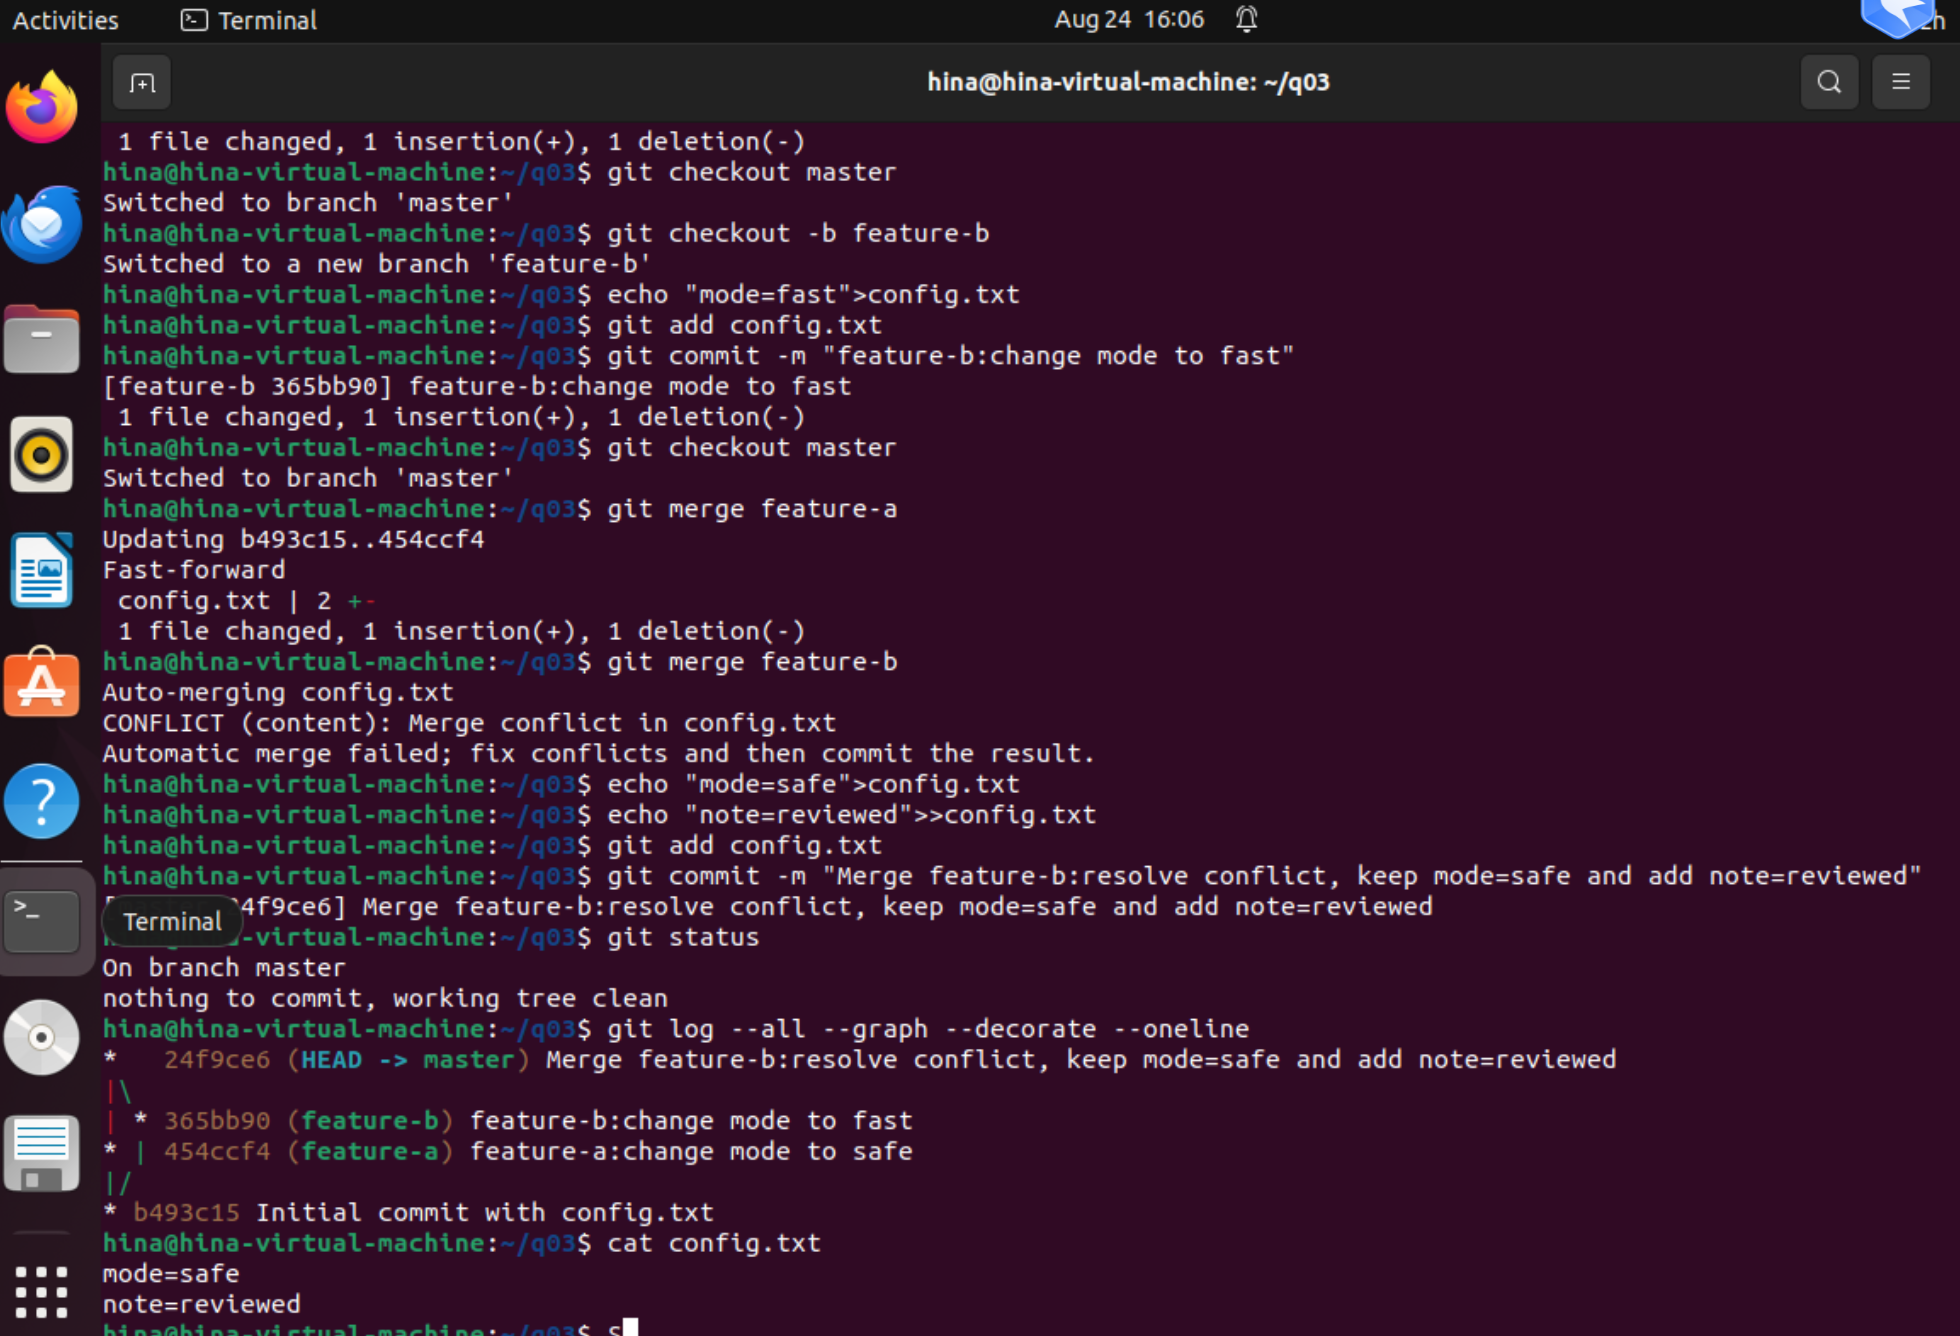
\includegraphics[width=15cm]{q03.png}\\[0.3cm]\\
\includegraphics[width=10cm]{q0302.png}\\[0.3cm]\\

% ============================================================
% 第4题
% ============================================================
\section{第4题：LaTeX 文档编译}
\label{sec:q4}

\subsection{题目要求}
在 \texttt{q04} 中创建 \texttt{report.tex}，补全内容并从命令行构建 PDF：
\begin{enumerate}
    \item 加入一个带编号和 \texttt{label} 的公式，并在正文中使用 \texttt{\textbackslash ref} 或 \texttt{\textbackslash eqref} 引用。
    \item 加入一个 2 行 2 列的表格，设置 \texttt{caption} 和 \texttt{label}，并在正文中引用该表。
    \item 使用 \texttt{latexmk -pdf -halt-on-error} 或 \texttt{xelatex} 生成 \texttt{report.pdf}。
    \item 确认 PDF 能打开，且交叉引用不显示 “??”。
\end{enumerate}

\subsection{实现过程}
编写 \texttt{report.tex}，包含以下关键元素：
\begin{lstlisting}[language=tex, caption=公式与表格的 LaTeX 代码]
\begin{equation}
\label{eq:sum}
\sum_{i=1}^{n} i = \frac{n(n+1)}{2}
\end{equation}

\begin{table}[h]
\centering
\begin{tabular}{|c|c|}
\hline
\textbf{Method} & \textbf{Time (ms)} \\
\hline
A & 120 \\
B & 85 \\
\hline
\end{tabular}
\caption{Performance comparison}
\label{tab:perf}
\end{table}
\end{lstlisting}

\subsection{踩坑记录}
\begin{enumerate}
    \item \textbf{缺少 \texttt{ctex.sty}：} 使用 \texttt{pdflatex} 编译时提示 \texttt{File 'ctex.sty' not found}。解决方法：安装 \texttt{texlive-latex-extra} 或改用 \texttt{xelatex}。
    \item \textbf{交叉引用显示 “??”：} 初次编译后，所有 \texttt{\textbackslash ref} 显示为 “??”。原因是只编译了一次。解决方法：执行两次 \texttt{xelatex report.tex}，第二次编译读取 \texttt{.aux} 文件中的标签信息。
\end{enumerate}

\subsection{验证结果}
编译后 \texttt{report.pdf} 正常打开，所有交叉引用显示正确的编号，无 “??” 出现。最终pdf截图如下\\
\includegraphics[width=15cm]{q04.png}\\[0.3cm]\\


% ============================================================
% 课后题（预留位置）
% ============================================================
\section{课后题}
以下为课后练习题目，来自课程教学网站的课后习题以及代码实例。

\subsection{第1题}
\label{sec:Q1}

\subsection*{题目内容}
根据教程，从命令行构建 PDF：
\begin{enumerate}
    \item 运用教程中的代码，初次生成LaTeX文档。
\end{enumerate}

\subsection*{实现过程}
编写 \texttt{Q1.tex}，包含以下关键元素：
\begin{lstlisting}[language=tex, caption=公式与表格的 LaTeX 代码]
\documentclass[a4paper, 12pt]{article}
\begin{document}
  My first LaTeX instance.
\end{document}
\end{lstlisting}

\subsection{第2题}
\label{sec:Q2}

\subsection*{题目内容}
根据教程，从命令行构建 PDF，实现章节功能：
\begin{enumerate}
    \item 运用教程中的代码，生成LaTeX文档。
\end{enumerate}

\subsection*{实现过程}
编写 \texttt{Q2.tex}，包含以下关键元素：
\begin{lstlisting}[language=tex, caption=公式与表格的 LaTeX 代码]
\documentclass[a4paper, 12pt]{article}

\begin{document}
  \title{Basic Structure}
  \author{Siri Pan}
  \date{\today}
  \maketitle

  \section{Introduction}
  This is the introduction.

  \section{Methods}

  \subsection{Stage 1}
  The first part of the methods.

  \subsection{Stage 2}
  The second part of the methods.

  \section{Results}
  Here are my results.
\end{document}
\end{lstlisting}
pdf截图\\

\includegraphics[width=15cm]{Q2.png}\\[0.3cm]\\

\subsection{第3题}
\label{sec:Q3}

\subsection*{题目内容}
根据教程，从命令行构建 PDF，实现字体大小的改变：
\begin{enumerate}
    \item 运用教程中的代码，生成LaTeX文档。
\end{enumerate}

\subsection*{实现过程}
编写 \texttt{Q3.tex}，包含以下关键元素：
\begin{lstlisting}[language=tex, caption=公式与表格的 LaTeX 代码]
\documentclass[a4paper, 12pt]{article}
\begin{document}
  \title{TITLE}
  \author{Siri Pan}
  \date{\today}
  \maketitle

normal size words {\tiny tiny words} \\
{\scriptsize scriptsize words}\\
{\footnotesize footnotesize words}\\
 {\small small words}\\
 {\large large words}\\
{\Large Large words} \\
{\LARGE LARGE words}\\ 
{\huge huge words}\\
\end{document}\end{lstlisting}
pdf截图\\

\includegraphics[width=15cm]{Q3.png}\\[0.3cm]\\


\subsection{第4题}
\label{sec:Q4}

\subsection*{题目内容}
根据教程，从命令行构建 PDF，生成一些数学公式：
\begin{enumerate}
    \item 运用教程中的代码，生成LaTeX文档。
\end{enumerate}

\subsection*{实现过程}
编写 \texttt{Q4.tex}，包含以下关键元素：
\begin{lstlisting}[language=tex, caption=公式与表格的 LaTeX 代码]
\documentclass[a4paper, 12pt]{article}
\usepackage[UTF8]{ctex}
\begin{document}
  \title{使用LaTeX生成数学公式}
  \author{Siri Pan}
  \date{\today}
  \maketitle

  \section{一些数学公式}
海伦公式：\\
$$p=\frac{a+b+c}{2}$$,$$S=\sqrt{p(p-a)(p-b)(p-c)}$$\\
一些不定积分公式：\\
$$\int 2xdx=x^2+c$$，$$\int 1dx=x+c$$\\
高斯求和：\\
$$\sum_{x=1}^n x=\frac{n(1+n)}{2}$$\\
ok呀也是测试成功了。
  \end{document}
\end{lstlisting}
pdf截图\\

\includegraphics[width=15cm]{Q4.png}\\[0.3cm]\\
\subsection{第5题}
\label{sec:Q5}

\subsection*{题目内容}
根据教程，从命令行构建 PDF，生成表格：
\begin{enumerate}
    \item 运用教程中的代码，生成LaTeX文档。
\end{enumerate}

\subsection*{实现过程}
编写 \texttt{Q5.tex}，包含以下关键元素：
\begin{lstlisting}[language=tex, caption=公式与表格的 LaTeX 代码]
\documentclass[a4paper, 12pt]{article}
\usepackage[UTF8]{ctex}
\begin{document}
  \title{使用LaTeX生成表格}
  \author{Siri Pan}
  \date{\today}
  \maketitle
 \section{生成表格}
 \begin{tabular}{|l|l|l|l|}
  \hline /  & Normal & Abnormal & Total \\
  \hline Sick & 20 & 180  & 200 \\
  \hline Healthy & 780 & 20 & 800 \\
\hline
  \end{tabular}\\
这其实是2025全国高考新I卷的独立性检验答题，最终的答案让许多人不敢落笔。\\
  \end{document}
\end{lstlisting}
pdf截图\\

\includegraphics[width=15cm]{Q5.png}\\[0.3cm]\\

\subsection{第6题}
\subsection*{题目内容}
写一条命令，把文件复制为带当天日期的备份文件名
\subsection*{实现过程}
\begin{lstlisting}[language=bash, caption=公式与表格的 LaTeX 代码]
cp document.txt "document_$(date +%Y-%m-%d).txt"
\end{lstlisting}\\
截图\\

\includegraphics[width=10cm]{Q6.png}\\[0.3cm]\\

\includegraphics[width=5cm]{Q602.png}\\[0.3cm]\\

\subsection{第7题}
\subsection*{题目内容}
使用 curl 获取 课程网站 的 HTML，并通过 grep 统计列出了多少讲。
\subsection*{实现过程}
\begin{lstlisting}[language=bash, caption=公式与表格的 LaTeX 代码]
curl -s https://missing.csail.mit.edu/ | grep -c '/2026/'
curl -s https://missing.csail.mit.edu/ | grep -cE 'href="/2026/[^"]+"'
\end{lstlisting}\\
第一行输出10，第二行输出9.\\
\subsection*{遇到的问题}
1.curl多次安装失败，在修改DNS后解决。\\
2.匹配到导航栏菜单<a href="/2026/">Course</a>导致输出为10而非9。\\
截图\\

\includegraphics[width=15cm]{Q7.png}\\[0.3cm]\\

\includegraphics[width=15cm]{Q702.png}\\[0.3cm]\\

\subsection{第8题}
\subsection*{题目内容}
jq 是处理 JSON 的强大工具。用 curl 获取示例数据 https://microsoftedge.github.io/Demos/json-dummy-data/64KB.json，再用 jq 提取 version 大于 6 的人员姓名。
\subsection*{实现过程}
\begin{lstlisting}[language=bash, caption=公式与表格的 LaTeX 代码]
curl -s https://microsoftedge.github.io/Demos/json-dummy-data/64KB.json | jq '.[] | select(.version > 6) | {name, version}'
\end{lstlisting}\\
截图，未完整列举\\
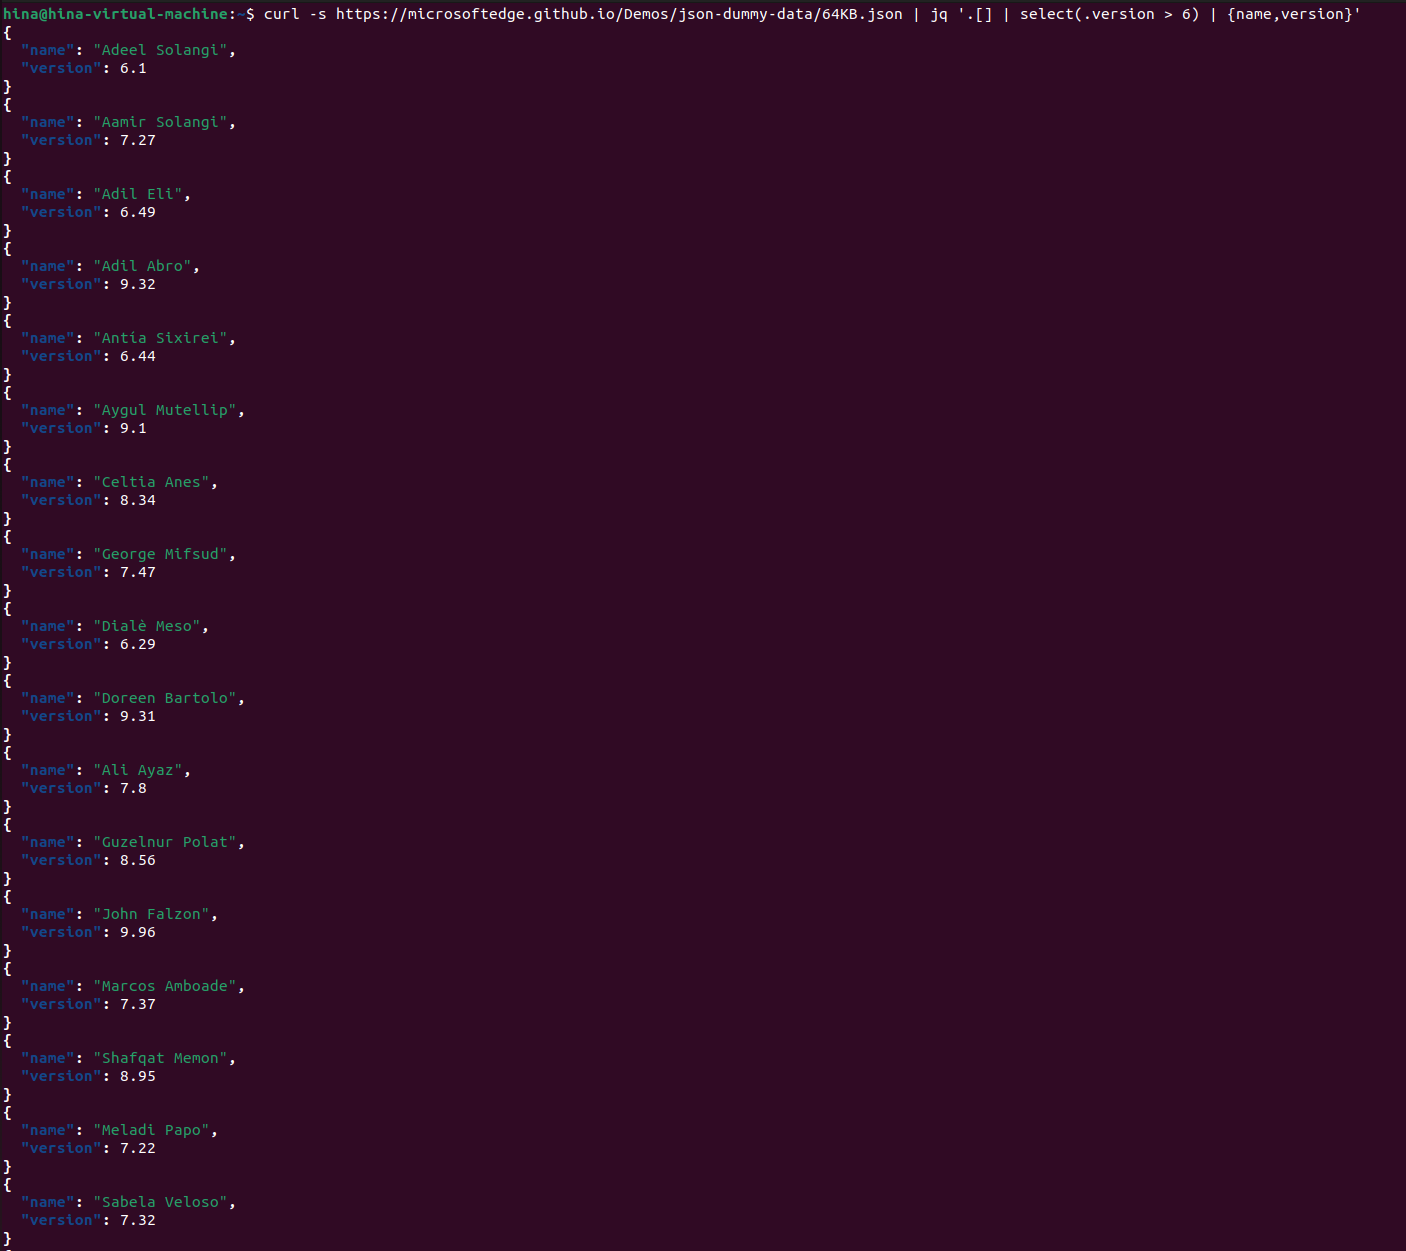
\includegraphics[width=15cm]{Q8.png}\\[0.3cm]\\


\subsection{第9题}
\subsection*{题目内容}
在脚本的 set 选项（flag）里加入 -x 会发生什么？写个简单脚本试试并观察输出。
\subsection*{实现过程}
\begin{lstlisting}[language=bash, caption=公式与表格的 LaTeX 代码]
#!/bin/bash
set -x 
name="Alice"
echo "Hello, $name"
set +x   
echo "Done"
\end{lstlisting}\\
截图，可知在开启调试模式时，会先输出将要运行的代码\\
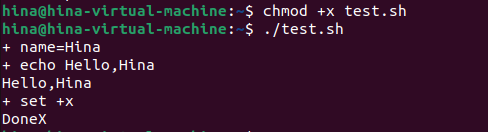
\includegraphics[width=15cm]{Q9.png}\\[0.3cm]\\

\subsection{第10题}
\subsection*{题目内容}
写一个脚本，接收文件名参数，用 test -f 或 [ -f ... ] 检查该文件是否存在，并根据结果输出不同提示。
\subsection*{实现过程}
\begin{lstlisting}[language=bash, caption=公式与表格的 LaTeX 代码]
#!/bin/bash
if [ -z "$1" ]; then
    echo "用法: $0 <文件名>"
    exit 1
fi

if test -f "$1"; then
    echo "文件 '$1' 存在且是一个普通文件。"
else
    echo "文件 '$1' 不存在或不是一个普通文件。"
fi
\end{lstlisting}\\
截图，使用了先前题目中创建的document.txt\\
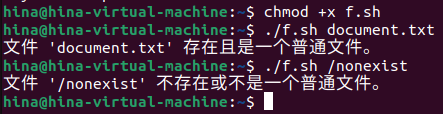
\includegraphics[width=15cm]{Q10.png}\\[0.3cm]\\

% ============================================================
% 个人感想
% ============================================================
\newpage
\section*{个人感想}
\addcontentsline{toc}{section}{个人感想}

通过本次实验，我对 Linux 环境下的一系列开发工具有了更加深入的理解。
我个人本身对Shell几乎完全不了解，只知道几条以前计导课上在虚拟机上使用过的命令。这节课也是我第一次使用LaTeX，面对新的问题我也踩了不少坑，最终在
不断地查询之后还是完成了问题，这让我收货颇丰。作为计算机专业的一名学生，这种挑战能让我在磨练中不断锻炼解决问题的能力以及提高专业知识的掌握，实在是意义非凡。
在使用LaTeX修改代码时对报告拥有未知的期待，我体会到了不断添加、修改的乐趣。


% ============================================================
% 总结
% ============================================================
\section*{总结}
\addcontentsline{toc}{section}{总结}

\begin{conclusionbox}
本次实验完成了四项独立任务，覆盖了 Shell 编程、日志分析、版本控制和 LaTeX 排版等核心技能：
\begin{enumerate}
    \item 熟练使用 Shell 命令进行文件操作、目录创建、权限设置和批量文件复制。
    \item 掌握了 \texttt{awk}、\texttt{sort}、\texttt{uniq}、\texttt{head} 等文本处理工具的管道组合使用。
    \item 理解了 Git 分支模型，并能够手动解决合并冲突。
    \item 掌握了 LaTeX 的公式、表格和交叉引用，并学会了使用自定义模板排版实验报告。
\end{enumerate}
通过本次实验，进一步提升了 Linux 环境下的开发效率和文档编写能力。
\end{conclusionbox}


\end{document}